\documentclass{article}

\usepackage{fancyhdr} % Required for custom headers
\usepackage{lastpage} % Required to determine the last page for the footer
\usepackage{extramarks} % Required for headers and footers
\usepackage[usenames,dvipsnames]{color} % Required for custom colors
\usepackage{graphicx} % Required to insert images
\usepackage{listings} % Required for insertion of code
\usepackage{courier} % Required for the courier font
\usepackage{lipsum} % Used for inserting dummy 'Lorem ipsum' text into the template
\usepackage{hyperref}
\usepackage{multirow}
\usepackage{tabularx}
\usepackage{longtable}
\usepackage{framed}
\usepackage{listings}
\usepackage{subfigure}
\usepackage{afterpage}
\usepackage{amsmath,amssymb}            
\usepackage{rotating}  
\usepackage{fancyhdr}
\usepackage{graphicx}
\usepackage{amsthm}
\usepackage[scriptsize]{caption} 
\hyphenation{a-gen-tiz-za-zio-ne}
% Margins
\topmargin=-0.45in
\evensidemargin=0in
\oddsidemargin=0in
\textwidth=6.5in
\textheight=9.0in
\headsep=0.25in

\linespread{1.1} % Line spacing

\lstset{
  numbers=left,
  stepnumber=5,    
  firstnumber=1,
  numberfirstline=true
}

% Set up the header and footer
\pagestyle{fancy}
\lhead{\hmwkAuthorName} % Top left header
\chead{\hmwkClass\ (\hmwkClassInstructor\ \hmwkClassTime): \hmwkTitle} % Top center head
\rhead{\firstxmark} % Top right header
\lfoot{\lastxmark} % Bottom left footer
\cfoot{} % Bottom center footer
\rfoot{Page\ \thepage\ of\ \protect\pageref{LastPage}} % Bottom right footer
\renewcommand\headrulewidth{0.4pt} % Size of the header rule
\renewcommand\footrulewidth{0.4pt} % Size of the footer rule

\setlength\parindent{0pt} % Removes all indentation from paragraphs

\usepackage{listings}
\usepackage{color}

\definecolor{dkgreen}{rgb}{0,0.6,0}
\definecolor{gray}{rgb}{0.5,0.5,0.5}
\definecolor{mauve}{rgb}{0.58,0,0.82}

\lstset{frame=tb,
  language=Java,
  aboveskip=3mm,
  belowskip=3mm,
  showstringspaces=false,
  columns=flexible,
  basicstyle={\small\ttfamily},
  numbers=none,
  numberstyle=\tiny\color{gray},
  keywordstyle=\color{blue},
  commentstyle=\color{dkgreen},
  stringstyle=\color{mauve},
  breaklines=true,
  breakatwhitespace=true
  tabsize=3
}

%----------------------------------------------------------------------------------------
%	DOCUMENT STRUCTURE COMMANDS
%	Skip this unless you know what you're doing
%----------------------------------------------------------------------------------------

% Header and footer for when a page split occurs within a problem environment
\newcommand{\enterProblemHeader}[1]{
\nobreak\extramarks{#1}{#1 continued on next page\ldots}\nobreak
\nobreak\extramarks{#1 (continued)}{#1 continued on next page\ldots}\nobreak
}

% Header and footer for when a page split occurs between problem environments
\newcommand{\exitProblemHeader}[1]{
\nobreak\extramarks{#1 (continued)}{#1 continued on next page\ldots}\nobreak
\nobreak\extramarks{#1}{}\nobreak
}




%----------------------------------------------------------------------------------------
%	NAME AND CLASS SECTION
%----------------------------------------------------------------------------------------

\newcommand{\hmwkTitle}{01 - Introduzione} % Assignment title
\newcommand{\hmwkDueDate}{Martedi,\ Marzo 15,\ 2016} % Due date
\newcommand{\hmwkClass}{Ingegneria del Software 1} % Course/class
\newcommand{\hmwkClassTime}{} % Class/lecture time
\newcommand{\hmwkClassInstructor}{Claudio Menghi} % Teacher/lecturer
\newcommand{\hmwkAuthorName}{} % Your name

%----------------------------------------------------------------------------------------
%	TITLE PAGE
%----------------------------------------------------------------------------------------

\title{
\vspace{2in}
\textmd{\textbf{\hmwkClass\\ \vspace{1cm} \hmwkTitle \vspace{1cm}}}\\
\normalsize\vspace{0.1in}\small{\hmwkDueDate}\\
\vspace{0.1in}\large{\textit{\hmwkClassInstructor\ \hmwkClassTime}}
\vspace{3in}
}


\theoremstyle{definition} 

\newtheorem{mydef}{Definizione}
\newtheorem{lemma}{Lemma}

\newtheorem{theorem}{Theorem}[section]

\author{\textbf{\hmwkAuthorName}}
\date{} % Insert date here if you want it to appear below your name

%----------------------------------------------------------------------------------------

\begin{document}

\maketitle

%----------------------------------------------------------------------------------------
%	TABLE OF CONTENTS
%----------------------------------------------------------------------------------------

%\setcounter{tocdepth}{1} % Uncomment this line if you don't want subsections listed in the ToC

\newpage
\tableofcontents
\newpage



%----------------------------------------------------------------------------------------
\section{Introduzione}
Questa lezione copre le  slides ``Classi come astrazioni" o in alternativa i capitoli  1- 2, 3, 4 e 5 del libro  Pellegrino Principe. “Java 8”.


\subsection{Le caratteristiche di Java}
Questa esercitazione ha come scopo quella di fornire una panoramica su Java e sulle sue caratteristiche fondamentali. In particolare Java \`e:
\begin{itemize}
\item \emph{Portabile} \`e la caratteristica principale di Java. L'obiettivo di Java \`e quello di consentire allo sviluppatore di  \emph{scrivere il programma una volta sola avendo la certezza che sar\`a possibile eseguirlo ovunque indipendentemenre dall'architettura della macchina su cui viene eseguito}. La filosofia di Java \`e quindi ``Write Once, Run Anywhere".
\item \emph{Compilato}: Java \`e un linguaggio compilato, ovvero viene ``tradotto" dal linguaggio di programmazione Java al linguaggio ``oggetto" bytecode. 
\item \emph{Orientato agli oggetti}: in un linguaggio orientato agli oggetti lo sviluppatore ragiona in termini di oggetti ovvero astrazioni dei concetti del mondo reale che lo sviluppatore vuole modellare\footnote{La filosofia \`e diversa da quella utilizzata per esempio quando si scrive in C dove gli ingredienti fondamentali sono le procedure. In un linguaggio procedurale le componenti fondamentali sono le funzioni ``procedure" che manipolano i dati del programma.}. In realt\`a Java \`e un linguaggio multi-paradigma dal momento che \`e anche procedurale, e se consideriamo Java 8 \`e anche funzionale (parzialmente).
\item \emph{Staticamente tipizzato}: un linguaggio \`e staticamente tipizzato quando \`e necessario associare ad ogni variabile un tipo.
\end{itemize}

\subsubsection{Java \`e portabile e compilato}
La caratteristica principale di Java \`e il fatto di essere portabile/platform indipendent. 
Se prendiamo per esempio C il compilatore genera un linguaggio ``oggetto" che \`e dipendente dalla macchina nel quale il compilatore viene eseguito. 
Il codice compilato pu\`o \textbf{solo} essere eseguito sulla piattaforma per il quale il codice \`e stato compilato.

In Java la fase di compilazione produce un codice intermedio chiamato \emph{byte-code} che pu\`o essere eseguito su macchine differenti supposto che ci sia installato sulla macchina un \emph{interprete} (Java Virtual Machine JVM) capace di capire il byte-code. 
In altre parole il byte-code \`e un codice intermedio prodotto dopo la compilazione. Il Byte-code differisce dal codice eseguibile (per esempio dai file ``.exe") dal momento che deve essere interpretato da una  Java Virtual Machine per essere eseguito.

\begin{figure}[h]
\centering
    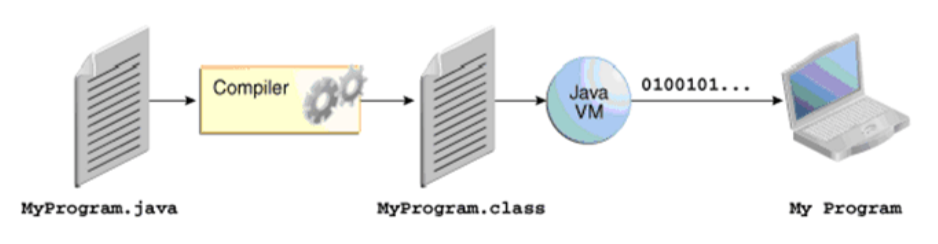
\includegraphics[width=0.7\textwidth]{Img/jvm-architecture.png}
    \caption{Java architecture}
    \label{JavaArchitecture}
\end{figure}

L'architettura del linguaggio Java \`e mostrata in Figura~\ref{JavaArchitecture}. Pi\`u precisamente,

\begin{itemize}
\item MyProgram.java: \`e il codice sorgente nativo dell'applicazione Java (Il file che contiene il nostro codice)
\item Compiler: (Compilatore) prende in input il nostro codice Java  (i nostri files \texttt{.java}), e produce dei file intermedi  (\texttt{.class}) ovvero i file contenenti il byte-code.
\item Java Virtual Machine: \`e l'interprete che deve essere installato sulla nostra macchina locale al fine di eseguire il byte-code. 
Il byte-code viene interpretato dalla Java Virtual Machine. Per questo motivo alcuni testi considerano Java anche come un linguaggio interpretato.
\end{itemize}

Per eseguire il vostro programma su una macchina \`e sufficiente che l'utente abbia installato una macchina virtuale: la Java Virtual Machine. 
In particolare, il \textbf{Java Run-time Environment} (JRE) contiene la macchina virtuale che consente di eseguire i programmi Java.  
JREs differenti sono associati a sistemi operativi differenti. 
Una volta istallata la JRE \`e possibile eseguire i class files generati.

Nota che, una volta generati, i class files possono essere eseguiti su ogni sistema cha abbia una Macchina Virtuale installata, indipendentemente dal sistema operativo su cui la macchina virtuale \`e eseguita.

Per compilare i file Java \`e necessario avere un tool di sviluppo Java: un \textbf{Java Development Kit} (JDK). 
Il JDK include la JRE e contiene un set di tool di svilupo che constentono di scrivere e compilare i tuoi programmi Java.




\subsubsection{Java \`e orientato agli oggetti}
La programmazione orientata agli oggetti implica un approccio alla programmazione completamente diverso rispetto ai normali lingguaggi procedurali. Gli oggetti sono entit\`a che hanno una ``vita propria" ed esistono indipendentemente dal come vengono utilizzate all'interno della nostra applicazione. In altre parole un 

\begin{mydef} \textbf{Oggetto} \`e un astrazione di un oggetto del mondo reale e ne descrive le caratteristiche  che sono di interesse allo sviluppatore.
\end{mydef}

In altre parole in un paradigma orientato agli oggetti lo sviluppatore descrive il mondo e i suoi oggetti e come il mondo evolve nel corso del tempo. 
In un paradigma procedurale lo sviluppatore specifica \textbf{come} risolvere un problema, mentre in un linguaggio orientato agli oggetti lo sviluppatore prima descrive ``il problema" e poi cerca una strategia per risolvere il probleam utilizzando il modello del mondo costruito.

Gli oggetti vengono creati partendo da dei modelli pi\`u generali chiamati classi. 

\begin{mydef} \textbf{Classi} sono dei \emph{tipi} definiti dall'utente che descrivono degli oggetti. In particolare descrivono l'oggetto, il suo \emph{stato} e come lo \emph{stato dell'oggetto} cambia in risposta a delle operazioni eseguite sull'oggetto.
\end{mydef}

Utilizzando un esempio automobilistico possiamo pensare alle classi come ai documenti di progetto di un autovettura, e agli oggetti come alle macchine realizzate partendo dai quei documenti. In altre parole le classi sono la teoria, gli oggetti sono particolari \textbf{istanze} di una specifica classe. 

Gli oggetti vengono creati con l'istruzione \textbf{new}. Per esempio l'istruzione seguente crea un nuovo oggetto di tipo Bike. 
\begin{lstlisting}
Bike myBike=new Bike();
\end{lstlisting}
La descrizione del tipo bike, ovvero la classe \texttt{Bike}, \`e presentata nel seguito.
\begin{lstlisting}[language=Java,escapechar=|]
public class Bike {

	public Bike(){
	}
}
\end{lstlisting}
Le classi sono definiti mediante la parola chiave (keyword) \texttt{class} e descrivono le caratteristiche dello stato di un oggetto e come lo stato pu\`o cambiare nel tempo.


\subsubsection{Java \`e staticamente tipizzato}
\begin{mydef} \textbf{Staticamente tipizzato} un linguaggio \`e staticamente tipizzato se ogni variabile \`e associata a un tipo: non \`e possibile creare una variabile senza un tipo.
\end{mydef}
\begin{lstlisting}
Bike bike1=new Bike();
\end{lstlisting}
Per esempio, l'istruzione precedente dichiara una variabile di tipo Bike con \textbf{identificatore} bike1, che \`e associata a un oggetto di classe Bike. 
In Java ogni variabile deve essere associata a un tipo.


\subsection{Variabili e tipi di riferimento}
Prima di discutere le variabili e i tipi di riferimento discutiamo per uno momento l'organizzazione della memoria in Java 

\begin{itemize}
\item \textbf{Stack} e \textbf{Heap}:  Lo stack e lo heap sono due aree di memoria che sono utilizzate per contenere le nostre variabili e i nostri oggetti.
\begin{itemize}
\item \textbf{Stack} \`e un area di memoria dove \`e possibile memorizzare informazioni. E' molto rapido e basato su un LIFO pattern.
\item \textbf{Heap} \`e uno spazio di memoria assegnabile al progetto e facilmente 
estendibile. 
\item Lo stack ha una dimensione fissa assegnata prima di eseguire il programma ``durante la fase di startup". Lo heap non ha uno specifico pattern, lo rende molto flessibile (\`e estendibile) ma \`e pi\`u lento. 
\end{itemize}


\begin{mydef} Una variabile \`e uno spazio di memoria che contiene un ``valore". 
\end{mydef}
Java \`e fortemente tipizzato (\emph{strongly typed}), quindi \emph{ogni variabile ha un tipo}. Il compilatore durante la compilazione controlla che le variabili siano utilizzate in maniera corretta in relazione al loro tipo.\\

\item \textbf{Variabili primitive}: le variabili primitive definiscono una ``cella di memoria" che contiene direttamente il valore della variabile. Le variabili primitive di Java sono:
\begin{itemize}
\item \emph{byte}: 8 bit, \emph{short}: 16 bit, \emph{int}: 32 bit, \emph{long}: 64 bit, \emph{float}: 32 bit, \emph{double}: 64 bit, \emph{char}: 16 bit \emph{boolean}: true/false
\end{itemize}
\item \textbf{Variabili riferimento}: le altre variabili contengono un riferimento alle aree di memoria cha contengono il ``valore": l'\textbf{oggetto}. I tipi di riferimento 1) possono essere definiti dall'utente mediante classi e interfacce, 2) includono gli array e le enumerazioni.
\item variabili primitive e di riferimento possono essere utilizzate nella stesso modo: come attributi, restituiti o passati a metodi.
\end{itemize}

Le \emph{variabili}:
\begin{itemize}
\item sono allocate sullo \emph{stack} a run-time quando si chiama il metodo su cui si sono dichiarate
\item si trovano nello heap quando rappresentano un attributo di un oggetto (vedremo in seguito).
\item se non sono attributi di un oggetto sono deallocate quando il sottoprogramma ritorna al chiamante
\end{itemize}
Gli \emph{oggetti}:
\begin{itemize}
\item sono allocati sullo heap.
\end{itemize} 



\textbf{Dove vengono allocati gli oggetti Java?}\\
Gli oggetti Java risiedono in una zona detta \emph{heap}. 
L'heap viene creato all'avvio della JVM e pu\'o cambiare dimensione durante l'esecuzione 
dell'applicazione. A discrezione della JVM viene eseguita l'operazione di ``\emph{garbage collection}'', che consiste nella rimozione degli oggetti non pi\`u utilizzabili dal programma per fare posto ad altri. 
Il componente che effettua tale operazione prende il nome di ``\emph{garbage collector}''.

\vspace{1cm}

\textbf{Quali sono le differenze tra i puntatori di C e le veriabili di riferimento di Java?}
\begin{itemize}
\item un riferimento non pu\`o essere de-allocato dall'utente, viene rimosso dal garbage collector
\item un riferimento non permette l'acceso all'indirizzo di memoria relativo ad un oggetto%TODO, ma a but a value that represent it
\item non \`e possibile effettuare operazioni aritmetiche sul riferimento, come \`e possibile sui puntatori nel linguaggio C
\end{itemize}







\subsubsection{Dichiarazione di una variabile}
Per dichiarare una variabile \`e sufficiente specificare il \emph{tipo} e un \emph{identificatore}, ovvero un nome simbolico utilizzato per riferirsi alla variabile\footnote{Java \`e case sensitive quindi caratteri in upper e lower case sono interpretati come caratteri differenti.}. \\
Per esempio, l'istruzione
\begin{lstlisting}[language=Java,escapechar=|]
int number;
\end{lstlisting}
dichiara una variabile di tipo primitivo ``\texttt{int}" con identificatore ``\texttt{number}", mentre l'istruzione
\begin{lstlisting}[language=Java,escapechar=|]
Car mycar;
\end{lstlisting}
dichiara una variabile di tipo riferimento ``\texttt{Car}" e con identificatore ``\texttt{mycar}".
La dichiarazione non alloca spazio per l'oggetto ma solo per il riferimento all'oggetto. \\

\emph{Qual'è la differenza tra tipi riferimenti e puntatori (e.g., i puntatori di C)?}\\
Ci sono varie differenze e similitudini tra riferimenti e puntatori. In genere un riferimento pu\`o essere interpretato come un puntatore ``ad alto livello", mentre la differenza fondamentale \`e per esempio i riferimenti non consentono l'utilizzo dell'aritmetica dei puntatori. 
\emph{Nei riferimenti l'indirizzo di memoria non \`e noto e non interessa}.

\subsubsection{Convenzione di notazione}
In Java i nomi di classi, variabili e metodi fanno uso della notazione a cammello (\emph{CamelCase}).
La notazione a cammello \`e costituita dalla giustapposizione delle parole che costituiscono l'identificativo, unite con l'iniziale di ogni parola maiuscola. 
La prima lettera dell'identificativo è maiuscola nel caso di classi e minuscola nel caso di metodi e attributi/variabili. 

\subsubsection{Inizializzazione di una variabile}
Una variabile non pu\`o essere usata senza essere inizializzata. Quando un attributo viene dichiarato gli viene assegnato un valore di default.

Il riferimento \`e assegnato inizialmente il valore \texttt{null}, per indicare che il riferimento non \`e ancora associato a un oggetto.
e variabili vengono inizializzate tramite l'operatore ``$=$''. Questo operatore assegna un valore ad una variabile.
Il tipo della variabile deve essere compatibile col tipo del valore.\\
Dichiarazione e inizializzazione possono essere effettuate in una o  pi\`u istruzioni, a discrezione
del programmatore.
\begin{lstlisting}[language=Java,escapechar=|]
// This characters are used to start a command
// declares the variable
int number;
// initializes a variable
number=0
\end{lstlisting}
Nell'esempio precedente la dichiarazione e l'assegnamento della variabile \texttt{number} sono
effettuati in istruzioni differenti.
\begin{lstlisting}[language=Java,escapechar=|]
// This characters are used to start a command
// declares and initializes the variable
int number=0
\end{lstlisting}
In quest'ultimo esempio nella medesima istruzione \texttt{number} viene dichiarata e inizializzata.

\subsubsection{Creazione di un nuovo oggetto}
La creazione di un nuovo oggetto si effettua con l'operatore new. Il metodo new costruisce un nuovo oggetto del tipo specificato e ritorna il suo riferimento
\begin{lstlisting}[language=Java,escapechar=|]
Car auto=new Car();
\end{lstlisting}
Effettuando new Car() viene creato un nuovo oggetto di tipo auto e viene ritornato il corrispettivo reference, che nel caso specifico viene assegnato alla variabile di riferimento auto mediante l'operatore di assegnamento $=$.

\subsection{Costruttori}
\begin{mydef} \textbf{Costruttore} un costruttore \`e un metodo della classe che ha il \emph{suo stesso nome} e \emph{non} ha tipi o valori di ritorno. Lo scopo del costruttore \`e quello di creare un nuovo ogggetto relativo a una classe.
\end{mydef}

\begin{itemize}
\item se una classe non ha un costruttore ne viene automaticamente uno di default senza argomenti che all'atto della creazione doll'oggetto richiama il costruttore di default senza argomenti della super classe.
\item se per\`o vengono creati dei costruttori il costruttore di default non risulta pi\`u disponibile a meno che definito dall'utente. 
\item l'uso di costruttori diversi permette di creare un tipo di oggetto passando argomenti diversi 
\end{itemize}

Un costruttore alloca + inizializza
\begin{itemize}
\item alloca lo spazio per gli attributi di tipo \emph{primitivo}
\item alloca lo spazio per i \emph{riferimenti} agli attributi definiti dall'utente
\item inizializza i riferimenti e gli attibuti. Se un riferimento non \`e inizializzato gli viene associato il valore null. Se una variabile numerica non \`e inizializzata gli viene associato il valore zero. Ai boolean viene assegnato il valore false
\end{itemize}


\subsection{Array}
\begin{itemize}
\item Un array \`e una variabile di tipo reference: contiene un reference a un area di memoria dove ci sono un insime di variabili dello stesso tipo.
\item un array ha una natura \emph{statica} mantiene la propria dimensione ovvero il numero di elementi che contiene.
\end{itemize}

Vari tipi di array possono essere dichiarati:
\begin{itemize}
\item array monodimensionali (anche noti come vettori)
\begin{itemize}
\item possono essere dichiarati come \texttt{type nomeVariabile[]} o come \texttt{type[] nomeVariabile} dove type indica il tipo di dato contenuti negli elementi dell'array mentre le parentesi poste dopo l'identificatore o dopo il tipo indicano che la variabile \`e di tipo array.
\item ovviamente in mancanza di \emph{inizializzazione} la dichiarazione di un array non alloca spazio per gli elementi dell'array
\item l'allocazione si realizza come \texttt{int[] i=new int[10];} dove 10 \'e il numero di elementi dell'array
\end{itemize}
\item Per quanto riguarda gli array multidimensionali la dichiarazione e l'inizializzazione avviene in maniera analoga \texttt{float[][] f=new float[10][10];}
\end{itemize}

\subsection{Semantic versioning}
Solitamente, ogni applicazione \`e associata a pi\`u versioni. Il numero di versione tiene traccia di come l'applicazione evolve nel tempo.
Per esempio Java 1.8 \`e una evoluzione di Java 1.7.

Solitamente a una applicazione \`e associato un numero di versione nella forma MAJOR.MINOR.PATCH, dove i campi hanno il seguente significato:
\begin{itemize}
\item MAJOR ogni volta che viene rilasciata una nuova versione con un cambiamento MAJOR significa che un cambiamento nelle API che rende l'applicazione incompatibile con la versione precedente \`e stata rilasciata. 
\item MINOR viene modificato ogni volta che vengono rilasciate nuove funzionalit\`a in una maniera backward compatibile
\item PATCH viene eseguita un attivit\`a di bug fixing in maniera backward compatibile.
\end{itemize}

Regole per l'uso di semantic versioning:
\begin{itemize}
\item il software DEVE dichiarare delle API pubbliche, precise e comprensibili;
\item MAJOR, MINOR e PATCH devono essere dei numeri NON negativi, e devono sempre incrementare. Quando la versione MAJOR (MINOR) viene incrementata il valore di MINOR e PATCH (PATCH) viene settato a zero;
\item una volta che una verione \`e rilasciata il contenuto della versione NON pu\`o essere modificato
\item la versione 0.y.z \`e la versione iniziale del software. Le API pubbliche devono essere considerate non stabili. Tutto pu\`o cambiare nel tempo.
\item la versione 1.0.0 \`e la prima versione del software che definisce le API pubbliche, da questo momento l'applicazione dipende dalle API pubbliche
\item il valore di PATCH deve essere incrementato solo se backward compatible bug fixes sono eseguiti. (Il bug fix corregge un comportamento scorretto)
\item il valore di MINOR deve essere incrementato se sono aggiunte funzionalit\'a introdotte nelle API pubbliche o se sono rimosse funzionalit\`a deprecate. Dopo aver incrementato MINOR \`e necessario settare PATCH a zero
\item il valore di MAJOR deve essere incrementato quando cambiamenti incompatibili sono introdotti nelle API pubbliche. PATCH e MINOR devono essere resettati a zero
\item una pre-release viene indicata utilizando un trattino seguita da un identificatore che specifica la patch version. Per esempio, 1.0.0-alpha.1, 1.0.0-0.3.7, 1.0.0-x.7.z.92. 
\end{itemize}

La versione iniziale del software \`e in genere la 0.1.0. Da li si inizia a utilizzare le regole sopra descritte.
\`E tempo di passare alla versione 1.0.0 quando:
\begin{itemize}
\item il software viene utilizzato in produzione;
\item si hanno delle API stabili che possono essere usati da altri.
\end{itemize}


Il lettore interessato pu\`o trovare informazioni addizionali in \url{http://semver.org/}.

\section{Esercizi}
L'obiettivo di questi esercizi \`e di chiarire le caratteristiche di Java prima descritte.

\subsection{Java \`e compilato ed \`e portabile}
Una variabile \`e una posizione di memoria che contiene un valore e pu\`o essere modificato. In Java esistono due tipi di variabili: 

Questi esercizi hanno come fine quello di mostrare il fatto che Java \`e un linguaggio compilato ed \`e portabile. 

\subsubsection{Esercizio 1}
\begin{framed}
\textbf{Esercizio 1}: Scrivere un programma Java che stampa a video: ``Benvenuto al corso di Ingegneria del Software"
\end{framed}

\begin{itemize}
\item \textbf{Creare un file Java}
\begin{itemize}
\item Aprire  TextEdit (per gli utenti mac), Blocco Note (per gli utenti Windows) of vi (for Linux per gli utenti linuz) .
\item (Per gli utenti Mac da TextEdit selezionare \textit{preferenze} $>$ \textit{Solo Testo} $>$ \textit{File} $>$ \textit{New} )
\item Scrivere il codice  Java seguente
\end{itemize}
\end{itemize}
\begin{lstlisting}
public class Welcome {	
    public static void main(String[] args){	
	 	System.out.println("Benvenuto al corso di Ingegneria del Software");
    }
}
\end{lstlisting}
\begin{itemize}
\item \textbf{Descrizione del file creato}
\begin{itemize}
\item il codice definisce una classe (\texttt{class}) chiamata  Welcome con un singolo metodo  \texttt{method} chiamato main
\item \texttt{public} \`e utilizzato per specificare che la classe \`e pubblica: \`e possibile accedervi dall'esterno, per esempio da altre classi.
\item la classe ha solo un metodo statico main
\item \texttt{void} specifica che il metodo non ritorna alcun valore
\item \texttt{static} specifica che il metodo \`e statico: pu\`o essere invocato senza instanziare l'oggetto di classe  (Welcome)
\item \texttt{main} \`e il ``metodo di partenza" che deve essere presente in almeno una classe affinch\`e l'applicazione sia eseguibile. 
\item \texttt{args} contiene il parametro (anche chiamato argomento) del metodo main.
 The parameters (also called arguments) are variables that can contains values that are passed to the method when is called. The parameters must have a type
\item \texttt{String[]} (array of String) is the type of the args parameter 
\item the arg parameter is used from main to obtain arguments that can be passed when the method is invoked from command line
\item \texttt{System.out.println} writes the specified text on the screen
\end{itemize}
\end{itemize}
\begin{itemize}
\item \textbf{Salvare il file} come Welcome.java (attenzione: non scegliere un nome differente e controllare che l'estensione del file sia .java).
\end{itemize}

\begin{itemize}
\item \textbf{Compilare il file Java}:
\begin{itemize}
\item aprire il Terminale (per gli utenti Mac e Linux) o il Command Propt (per gli utenti Windows)
\item portarsi nella cartella dove si trova il file creato mediante i seguenti comandi
\begin{itemize}
\item per gli utenti  Mac and Linux Users \`e possibile aprire e chiudere una cartella mediante i comandi \emph{cd}, e \emph{cd ..}, rispettivamente e mostrare il contenuto di una cartella con il comando \emph{ls}) 
\end{itemize}
\item Digitare \texttt{javac Welcome.java}
\item il comando \texttt{javac}  \textbf{compila} il file Welcom.jar file e genera un file .class (o un jar) che contiene il bytecode file che \`e possibile eseguire su qualunque piattaforma\footnote{Ricordiamo che il bytecode \`e una rappresentazione intermedia che pu\`o essere interpretata da una macchina virtuale Virtual Machine.}. Questo processo supporta la  \textbf{portabilit\a`}. 
\item \emph{Per eseguire con successo il comando \emph{javac} \`e necessario avere una JDK (Java Development Kit) istallata sul proprio pc\footnote{Nota che la JDK include anche il Java Run-Time Environment}.} La JDK permette quindi di  \emph{compilare} e \emph{eseguire} il programma creato.
\end{itemize}
\end{itemize}

\begin{itemize}
\item \textbf{Eseguire il file Java}
\begin{itemize}
\item il java bytecode (.class) pu\`o essere eseguito in qualsiasi architettura dove \`e installata una Virtual Machine (la quale fornisce un  \textbf{interprete} per il $Java$ bytecode) . In particolare la Java JRE fornisce questa Virtual Machine.
\item per eseguire il file bytecodefile eseguire il comando \texttt{java Welcome}
\item questo comando esegue il   \texttt{Main} method della classe Welcome
\end{itemize}
\end{itemize}




\subsubsection{Esercizio 2}
\begin{framed}
\textbf{Esercizio 2}: Richiedere all'utente di inserire il proprio nome (per esempio Carlo) e stampare ``Ciao Carlo, Benvenuto al corso di Ingegneria del Software"
\end{framed}
\begin{itemize}
\item \textbf{Creare un file Java}
\begin{itemize}
\item crea un file Java con nome \texttt{WelcomeWithName}
\item scrivere il seguente codice Java
\end{itemize}
\end{itemize}
\begin{lstlisting}[
    language=Java,escapechar=|]
import java.util.Scanner;

public class WelcomeWithName {
	public static void main(String[] args){
		Scanner scanner = new Scanner(System.in); |\label{line:scanner}|
		System.out.println("Inserisci il tuo nome:");
		String nome = scanner.nextLine();
		scanner.close();
		String welcome = "Benvenuto al corso di Ingegneria del Software";
		System.out.println("Ciao " + nome + ", " + welcome);
	}
}
\end{lstlisting}
\begin{itemize}
\item \textbf{Descrizione del file creato}
\begin{itemize}
\item \texttt{import} is used to import the \texttt{class} Scanner which is contained in the \texttt{java.util} package
\item \texttt{new} creates (\texttt{instantiate}) a new Scanner Object
\item \texttt{scanner.nextLine()} reads the next of the current line
\item \texttt{scanner.close()} close the scanner
\end{itemize}
\end{itemize}

\begin{itemize}
\item  \textbf{Compilare ed eseguire il file creato}
\begin{itemize}
\item \texttt{javac WelcomeWithName.java}
\item \texttt{java WelcomeWithName}
\end{itemize}
\end{itemize}

\subsection{Java \`e orientato agli oggetti e staticamente tipizzato}


\subsubsection{Esercizio 1}
\begin{framed}
\textbf{Esercizio 2}: Modellizzare in Java una bicicletta, una bicicletta (in un particolare istante temporale) ha una determinata velocit\`a, che dipende dalla marcia inserita e dal ritmo di pedalata
\end{framed}

Per progettare le vostre classi in Java \`e necessario rispondere a due quesiti:
\begin{itemize}
\item Come \`e possibile descrivere lo \emph{stato} degli oggetti relativi a una determinata classe?
\item Quali sono le \emph{funzionalit\`a} che gli oggetti di una determinata classe devono fornire?
\end{itemize}


\begin{lstlisting}[language=Java,escapechar=|]
// defines a public class called Bike 
// the name of the class usually starts with an upper case letter
public class Bike {
	
	// The attributes of the class are used to describe the state of the class and are usually private or protected 
	// The attributes of the class usually start with lower case letters
	private int gear=1; //default 1
	private int cadence; //default 0
	private int speed; //default 0
	
	// is the constructor of the class which allows to create a new Bike
	// the constructor has the same name of the class and does not have a return type
	public Bike(){
	}
}
\end{lstlisting}


\subsubsection{Esercizio 2}
\begin{framed}
\textbf{Esercizio 2}: Implementare un client per la classe bicicletta
\end{framed}
Un Java si utilizza l'espressione client per indicare una generica classe, che utilizza la classe da noi progettata (nel nostro caso la classe Bicicletta). 


\begin{lstlisting}[language=Java,escapechar=|]
public class Client {
	
	public static void main(String[] args)
    {
        Bike bike1; // defines a new reference (pointer) of class Bike with a predefined value null
        bike1 = new Bike(); // instantiate  the object
        // the instruction new Bike() creates a new object of type Bike and returns the reference to this object which is assigned to the reference bike1
        // when the method new is invoked, the VM allocates dynamically the quantity of memory which is sufficient to contain the Bike object
        Bike bike2 = new Bike(); // defines and instantiate a new object of class Bike
     }
}
\end{lstlisting}
\begin{itemize}
\item compilare ed eseguire il programma
\end{itemize}

\begin{itemize}
\item 
\textbf{Quesiti:}\\
\begin{itemize}
\item Qual'\`e lo stat dell'oggetto dopo l'istruzione \emph{Bike bike1;}?\emph{l'oggetto non ha uno stato, visto che non esiste esiste solamente il suo reference.}
\item Qual'\`e lo stato dell'oggetto  \texttt{bike1} dopo l'istruzione  \texttt{bike1 = new Bike()}? \texttt{gear=1}, \texttt{cadence=0}, \texttt{speed=0}
\item Qual'\`e lo stato dell'oggetto  \texttt{bike1} dopo l'istruzione \texttt{bike2 = new Bike()}? \texttt{gear=1}, \texttt{cadence=0}, \texttt{speed=0}
\item Qual'\`e lo stato dell'oggetto  \texttt{bike1} dopo l'istruzione \texttt{bike2 = new Bike()}? \texttt{gear=1}, \texttt{cadence=0}, \texttt{speed=0}
\end{itemize}
\end{itemize}



\subsubsection{Esercizio 3}
\begin{lstlisting}[language=Java,escapechar=|]
public class Client {
	
	public static void main(String[] args)
    {
        Bike bike1; 
        bike1 = new Bike();
        Bike bike2 = new Bike(); 
        
        // == compare the reference of the Bike1 with the reference of the Bike2
        System.out.println(bike1==bike2);
     }
}
\end{lstlisting}

\begin{itemize}
\item Che cosa stampa l'istruzione  \texttt{bike1==bike2}? \emph{false, visto che i references ai due oggetti  \texttt{bike1} e \texttt{bike2} si riferiscono al medesimo oggetto}
\end{itemize}


\subsubsection{Esercizio 4}
\begin{framed}
\textbf{Esercizio 4}: Aggiungere alla bicicletta una funzionalit\`a che permette all'oggetto di stampare il suo stato
\end{framed}

\begin{lstlisting}[language=Java,escapechar=|]
// defines a public class called Bike 
// the name of the class usually starts with an upper case letter
public class Bike {
	
	// The attributes of the class are used to describe the state of the class and are usually private or protected 
	// The attributes of the class usually start with lower case letters
	private int gear=1; //default 1
	private int cadence; //default 0
	private int speed; //default 0
	
	// is the constructor of the class which allows to create a new Bike
	// the constructor has the same name of the class and does not have a return type
	public Bike(){
	}
	
	public void printState(){
	    // + is the String concatenation operator
	    // the int gear, speed and cadence are automatically converted into String
		System.out.println("gear: "+ gear + ", speed: "+speed+ ", cadence: "+cadence);
	}
}
\end{lstlisting}

\subsubsection{Esercizio 5}
\begin{framed}
\textbf{Esercizio 5}: Cambiare il package delle classi e compilare
\end{framed}
\begin{lstlisting}[language=Java,escapechar=|]
package transport;

// defines a public class called Bike 
// the name of the class usually starts with an upper case letter
public class Bike {
	
	// The attributes of the class are used to describe the state of the class and are usually private or protected 
	// The attributes of the class usually start with lower case letters
	private int gear=1; //default 1
	private int cadence; //default 0
	private int speed; //default 0
	
	// is the constructor of the class which allows to create a new Bike
	// the constructor has the same name of the class and does not have a return type
	public Bike(){
	}
	
	public void printState(){
	    // + is the String concatenation operator
	    // the int gear, speed and cadence are automatically converted into String
		System.out.println("gear: "+ gear + ", speed: "+speed+ ", cadence: "+cadence);
	}
}
\end{lstlisting}

\begin{lstlisting}[language=Java,escapechar=|]
// imports the class Bike inside the package transport
import transport.Bike;

public class Client {
	
	public static void main(String[] args)
    {
        Bike bike1; 
        bike1 = new Bike();
        Bike bike2 = new Bike(); 
        
        // == compare the reference of the Bike1 with the reference of the Bike2
        System.out.println(bike1==bike2);
        // invokes the method print state of the object bike1       
          bike1.printState();
          // invokes the method print state of the object bike2
            bike2.printState();

     }
}
\end{lstlisting}

If we change folder of the bike class we have to change the package

\subsection{Eclipse Integrated Development Environment  (20 min)}
La gestione di un progetto man mano che la complessit\`a aumenta diventa sempre pi\`u difficile. Per questo, nello sviluppo softeware  Integrated Development Environment ($IDE$) sono comunemente utilizzati. Gli $IDE$s rimuovono alcune delle difficolt\`a solitamente incontrate nel processo di sviluppo e forniscono funzionalit\`a aggiuntive come il completamento automatico del codice. In questo corso e in paricolare nel laboratorio useremo $Eclipse IDE$ come ambiente di sviluppo\footnote{$Netbeans$ one of the most used competitor of $Eclipse$}.  

\subsubsection{Esercizio 6}
\begin{framed}
\textbf{Esercizio 6}: Crea il tuo primo progetto in Eclipse
\end{framed}

\begin{itemize}
\item \textbf{Creare un progetto in eclipse}
\begin{itemize}
\item apri $Eclipse$
\item non appena $Eclipse$ si avvia richiede all'utente di selezionare il $Workspace$. Il $Workspace$ \`e l'are di lavoro dell'utente, contiene i file creati etc. L'utente pu\`o definire varit $Workspace$s ognuno dei quali pu\`o contenere pi\`u progetti.
\item clicca su $Workbench$ 
\item \texttt{File} $>$ \texttt{New} $>$ \texttt{Project} $>$ \texttt{Maven Project}
\item seleziona \texttt{Create a simple project}
\item digita \texttt{IngegneriaDelSoftware1} as Group Id and \texttt{Esercitazione1} as Artifact Id
\item scegli \texttt{finish}
\item Quando create il vostro nuovo progetto Maven (Maven\footnote{Maven sar\`a spiegato nel corso del laboratorio.}) in Eclipse, eclise crea automaticamente la struttura del vostro progetto. In particolare, 
\begin{itemize}
\item $src/main/java$ contiene il codice sorgente Java dell'applicazione in via di sviluppo.
\item $src/main/resources$ contiene le ``risorse" utilizzate dalla vostra applicazione, file di configurazione etc
\item $src/test/java$ contiene le cassi usate per testare la vostra applicazione
\item $src/test/resources$ contiene le risorse necessarie a testare la vostra applicazione
\end{itemize}
\end{itemize}
\end{itemize}



\begin{itemize}
\item \textbf{Creare un package}
\begin{itemize}
\item tasto destro su \texttt{src/main/java} $>$ New $>$ package 
\item scegliere il nome del package ($esercitatione1$)
\item press finish
\end{itemize}
\end{itemize}

\begin{itemize}
\item \textbf{Creare una nuova classe in Eclipse}
\begin{itemize}
\item tasto destro sul package dove si desidera creare la classe  $>$ New $>$ class 
\item scegliere il nome della classe (\texttt{Bike})
\item scegliere i modificatori di accesso della classe etc...
\item premere finish
\end{itemize}
\end{itemize}
Come noti  Eclipse automaticamente aggiunge il package, gli identificatori etc

\begin{itemize}
\item \textbf{Running a project in Eclipse}
\begin{itemize}
\item cliccare con il tasto destro sulla classe che si desidera eseguire (\emph{deve contenere il metodo  main})
\item Run As $>$ Java Application
\end{itemize}
\end{itemize}

\begin{itemize}
\item \textbf{Che cosa succede?}
\begin{itemize}
\item se apriamo il workspace notiamo che il nostro progetto contiene varie cartelle: 
\begin{itemize}
\item src: contiene i file sorgenti delle nostre applicazioni (\texttt{.java} files)
\item target: contains i file che contengono il bytecode (\texttt{.class} files) che sono generati dopo aver eseguito la procedura appena descritta. La compilazione ed esecuzione \`e resa trasparente all'utente
\end{itemize}
\end{itemize}
\end{itemize}

\subsection{Java \`e orientato agli oggetti 2 e staticamente tipizzato}

\subsubsection{Esercizio 7}
\begin{framed}
\textbf{Esercizio 7}: Deve essere possibile monitorare la velocit\`a la marcia inserita e il ritmo di pedalata di una bicicletta 
\end{framed}


\begin{lstlisting}[language=Java,escapechar=|]
package esercitatione1;


//defines a public class called Bike 
//the name of the class usually starts with an upper case letter
public class Bike {
	
	// The attributes of the class are used to describe the state of the class and are usually private or protected 
	// The attributes of the class usually start with lower case letters
	private int gear=1; //default 1
	private int cadence; //default 0
	private int speed; //default 0
	
	// is the constructor of the class which allows to create a new Bike
	// the constructor has the same name of the class and does not have a return type
	public Bike(){
	}
	
	public void printState(){
	    // + is the String concatenation operator
	    // the int gear, speed and cadence are automatically converted into String
		System.out.println("gear: "+ gear + ", speed: "+speed+ ", cadence: "+cadence);
	}
	
	// returns the gear of the bike
	public int getGear(){
		return this.gear;
	}

	// returns the cadence of the bike
	public int getCadence(){
		return this.cadence;
	}
	
	// returns the speed ok the bike
	public int getSpeed(){
		return this.speed;
	}
}
\end{lstlisting}

Il ``Monitoring" di un oggetto \`e eseguito mediante i metodi getters.\\
Command tricks:
\begin{itemize}
\item il comando Control + Space permette di completare automaticamente il testo e fornisce suggerimenti al riguardo
\end{itemize}


\begin{lstlisting}[language=Java,escapechar=|]
package esercitatione1;

public class Client {

	public static void main(String[] args) {

		Bike bike1;
		bike1 = new Bike();
		Bike bike2 = new Bike();

		// == compare the reference of the Bike1 with the reference of the Bike2
		System.out.println(bike1 == bike2);
		// invokes the method print state of the object bike1
		bike1.printState();
		// invokes the method print state of the object bike2
		bike2.printState();

		System.out.println(bike1.getCadence());
	}

}

\end{lstlisting}


\subsubsection{Esercizio 8}
\begin{framed}
\textbf{Esercizio 8}: Deve essere possibile incrementare la marcia inserita e il ritmo di pedalata, in tal caso la velocit\`a deve aumentare di conseguenza
\end{framed}

\begin{lstlisting}[language=Java,escapechar=|]
package esercitatione1;

//defines a public class called Bike 
//the name of the class usually starts with an upper case letter
public class Bike {

	// The attributes of the class are used to describe the state of the class
	// and are usually private or protected
	// The attributes of the class usually start with lower case letters
	private int gear=1; // default 1
	private int cadence; // default 0
	private int speed; // default 0

	// is the constructor of the class which allows to create a new Bike
	// the constructor has the same name of the class and does not have a return
	// type
	public Bike() {
	}

	public void printState() {
		// + is the String concatenation operator
		// the int gear, speed and cadence are automatically converted into
		// String
		System.out.println("gear: " + gear + ", speed: " + speed
				+ ", cadence: " + cadence);
	}
    
    // changes the cadence of the bike
	public void changeCadence(int cadence) {
		this.cadence = cadence;
		updateSpeed();
	}

	// increment the gear
	public void incrementGear() {
		this.gear++;
		this.updateSpeed();
	}

	// decrement the gear
	public void decrementGear() {
		this.gear--;
		this.updateSpeed();
	}

	// every time the cadence or the gear changes the speed is updated
	// the method is private and cannot be invoked from other external classes
	private void updateSpeed(){
		this.speed = this.gear * this.cadence; 
	}
	
	// returns the gear of the bike
	public int getGear() {
		return this.gear;
	}

	// returns the cadence of the bike
	public int getCadence() {
		return this.cadence;
	}

	// returns the speed ok the bike
	public int getSpeed() {
		return this.speed;
	}
}
\end{lstlisting}


\begin{lstlisting}[language=Java,escapechar=|]
package esercitatione1;

public class Client {

	public static void main(String[] args) {

		Bike bike1;
		bike1 = new Bike();
		Bike bike2 = new Bike();

		// == compare the reference of the Bike1 with the reference of the Bike2
		System.out.println(bike1 == bike2);
		// invokes the method print state of the object bike1
		bike1.printState();
		// invokes the method print state of the object bike2
		bike2.printState();

		bike1.printState();
		bike1.incrementGear();
		bike1.printState();
		
		bike1.changeCadence(10);
		bike1.printState();
		
	}
}
\end{lstlisting}

\begin{itemize}
\item \textbf{Quesiti}
\begin{itemize}
\item Qual'\`e lo stato dell'oggetto \texttt{bike1} dopo che l'istruzione \texttt{bike1.incrementGear();} \`e eseguita? 
\texttt{gear=2}, \texttt{cadence=0}, \texttt{speed=0}.
\item Qual'\`e lo stato dell'oggetto  \texttt{bike1} dopo che l'istruzione \texttt{bike1.changeCadence(10);} \`e eseguita? 
\texttt{gear=2}, \texttt{cadence=10}, \texttt{speed=0}.
\end{itemize}
\end{itemize}

\subsubsection{Esercizio 9}
\begin{framed}
\textbf{Esercizio 9}: La classe di biciclette considerate ha $6$ marce
\end{framed}
\begin{lstlisting}[language=Java,escapechar=|]
package esercitatione1;

//defines a public class called Bike 
//the name of the class usually starts with an upper case letter
public class Bike {

	// static specifies that this variable is shared from all the objects
	// The final modifier indicates that the value of this field cannot change.
 	// The static modifier, in combination with the final modifier, is also used to define constants. 
	private static final int MAX_GEAR = 6;
	private static final int MIN_GEAR = 1;

	// The attributes of the class are used to describe the state of the class
	// and are usually private or protected
	// The attributes of the class usually start with lower case letters
	private int gear = 1; // default 1
	private int cadence; // default 0
	private int speed; // default 0

	// is the constructor of the class which allows to create a new Bike
	// the constructor has the same name of the class and does not have a return
	// type
	public Bike() {
	}

	public void printState() {
		// + is the String concatenation operator
		// the int gear, speed and cadence are automatically converted into
		// String
		System.out.println("gear: " + gear + ", speed: " + speed
				+ ", cadence: " + cadence);
	}

	// changes the cadence of the bike
	public void changeCadence(int cadence) {
		this.cadence = cadence;
		updateSpeed();
	}

	// increment the gear
	public void incrementGear() {
		if (gear < MAX_GEAR) {
			gear++;
			updateSpeed();
		}
	}

	// decrement the gear
	public void decrementGear() {
		if (gear > MIN_GEAR) {
			gear--;
			updateSpeed();
		}
	}

	// every time the cadence or the gear changes the speed is updated
	// the method is private and cannot be invoked from other external classes
	private void updateSpeed() {
		this.speed = this.gear * this.cadence;
	}

	// returns the gear of the bike
	public int getGear() {
		return this.gear;
	}

	// returns the cadence of the bike
	public int getCadence() {
		return this.cadence;
	}

	// returns the speed ok the bike
	public int getSpeed() {
		return this.speed;
	}
}
\end{lstlisting}




\subsection{Variabili e tipi di riferimento}

\subsubsection{Esercizio 10}
\begin{framed}
\textbf{Esercizio 10}: Analizzare che cosa succede eseguendo il seguente codice
\end{framed}
\begin{lstlisting}[language=Java,escapechar=|]
package esercitatione1;

public class Client {

	public static void main(String[] args) {

        // dichiaro una variabile di tipo reference con identificativo bike1
        Bike bike1;
        // creo un nuovo oggetto di tipo Bike e assegno il reference ritornato alla variabile bike1
        bike1 = new Bike();
        // creo un nuovo oggetto di tipo Bike e assegno il reference ritornato alla variabile bike2
        Bike bike2 = new Bike();
        
        // vengono stampati due reference diversi relativi alle variabili bike1 e bike2
    	System.out.println(bike1);
    	System.out.println(bike2);
    	
    	// copia il reference contenuto nella variabile bike2 nella variabile bike1
    	bike1 = bike2;
    
       // vengono stampati i due reference
       System.out.println(bike1);
       System.out.println(bike2);	
       }
}
\end{lstlisting}
Per avere una visualizzazione migliore di quanto accade utilizzeremo il debugger di eclipse. Il debugger vi consente di eseguire passo passo il vostro codice e vi assiste nell'individuazione e nella correzioni di errore in un programma.

\begin{itemize}
\item cliccare con il tasto destro del mouse sulla barra vertical a fianco a \texttt{public static void main}
\item cliccare su \texttt{toggle breakpoing}
\item cliccare con il tasto destro sulla nostra classe (Client.java)
\item cliccare su debug as Java Application
\item se viene chiesto se aprire il perspective di debug rispondere Yes
\end{itemize}
Nella View variables \`e possibile vedere passo passo le variabili sullo stack. Se una variabile \`e di tipo reference \`e possibile esplorare il corrispondente oggetto (e di conseguenza lo heap)

\`E possibile proseguire nell'esecuzione del codice (un passo alla volta) premendo sul pulsante step over (la freccia gialla posta al centro delle le tre in alto a sinistra)\footnote{Un utilizzo pi\`u dettagliato del debugger verr\`a descritto nel corso del laboratorio}.

\subsubsection{Esercizio 11}
\begin{framed}
\textbf{Esercizio 11}: Analizzare che cosa succede eseguendo il seguente codice
\end{framed}
\begin{lstlisting}[language=Java,escapechar=|]
package esercitatione1;

public class Client {

	public static void creatingANewBike() {
		// dichiaro una variabile di tipo reference con identificativo bike1
		Bike bike1;
		// creo un nuovo oggetto di tipo Bike e assegno il reference ritornato
		// alla variabile bike1
		bike1 = new Bike(4, 5);
	}

	public static void main(String[] args) {

		// dichiaro una variabile di tipo reference con identificativo bike1
		Bike bike1;
		// creo un nuovo oggetto di tipo Bike e assegno il reference ritornato
		// alla variabile bike1
		bike1 = new Bike(4, 5);
		// creo un nuovo oggetto di tipo Bike e assegno il reference ritornato
		// alla variabile bike2
		Bike bike2 = new Bike(2, 3);

		// vengono stampati due reference diversi relativi alle variabili bike1
		// e bike2
		System.out.println(bike1);
		System.out.println(bike2);

		// copia il reference contenuto nella variabile bike2 nella variabile
		// bike1

		bike1 = bike2;

		// vengono stampati i due reference
		System.out.println(bike1);
		System.out.println(bike2);
		
		creatingANewBike();
    }
}
\end{lstlisting}


\subsection{Costruttori}
\subsubsection{Esercizio 12}
\begin{framed}
\textbf{Esercizio 12}: Modificare la classe bicibletta affinch\`e sia possibile creare una bicicletta con un numero di marce  un dato ritmo di pedalata
\end{framed}

\begin{lstlisting}[language=Java,escapechar=|]
package esercitatione1;

//defines a public class called Bike 
//the name of the class usually starts with an upper case letter
public class Bike {

	// static specifies that this variable is shared from all the objects
	// The final modifier indicates that the value of this field cannot change.
 	// The static modifier, in combination with the final modifier, is also used to define constants. 
	private static final int MAX_GEAR = 6;
	private static final int MIN_GEAR = 1;

	// The attributes of the class are used to describe the state of the class
	// and are usually private or protected
	// The attributes of the class usually start with lower case letters
	private int gear = 1; // default 1
	private int cadence; // default 0
	private int speed; // default 0

	// is the constructor of the class which allows to create a new Bike
	// the constructor has the same name of the class and does not have a return
	// type
	// gear and cadence are the intial values of the gear and the cadence
	public Bike(int gear, int cadence) {
		
		// this allows to refer to the variable gear of THIS class, otherwise gear refers to the variable passed as parameter
		this.gear=gear;
		this.cadence=cadence;
		this.updateSpeed();
	}

	public void printState() {
		// + is the String concatenation operator
		// the int gear, speed and cadence are automatically converted into
		// String
		System.out.println("gear: " + gear + ", speed: " + speed
				+ ", cadence: " + cadence);
	}

	// changes the cadence of the bike
	public void changeCadence(int cadence) {
		this.cadence = cadence;
		updateSpeed();
	}

	// increment the gear
	public void incrementGear() {
		if (gear < MAX_GEAR) {
			gear++;
			updateSpeed();
		}
	}

	// decrement the gear
	public void decrementGear() {
		if (gear > MIN_GEAR) {
			gear--;
			updateSpeed();
		}
	}

	// every time the cadence or the gear changes the speed is updated
	// the method is private and cannot be invoked from other external classes
	private void updateSpeed() {
		this.speed = this.gear * this.cadence;
	}

	// returns the gear of the bike
	public int getGear() {
		return this.gear;
	}

	// returns the cadence of the bike
	public int getCadence() {
		return this.cadence;
	}

	// returns the speed ok the bike
	public int getSpeed() {
		return this.speed;
	}
}
\end{lstlisting}

\begin{lstlisting}[language=Java,escapechar=|]
package esercitatione1;

public class Client {

	public static void main(String[] args) {

		Bike bike1;
		bike1 = new Bike(3, 2);
		Bike bike2 = new Bike(1, 2);

		// == compare the reference of the Bike1 with the reference of the Bike2
		System.out.println(bike1 == bike2);
		// invokes the method print state of the object bike1
		bike1.printState();
		// invokes the method print state of the object bike2
		bike2.printState();

		bike1.printState();
		bike1.incrementGear();
		bike1.printState();
		bike1.changeCadence(10);
		bike1.printState();
	    }
}
\end{lstlisting}
\textbf{Quesiti:}\\
\begin{itemize}
\item Qual'\`e lo stato dell'oggetto \texttt{bike1} dopo che l'istruzione   \texttt{bike1=new Bike(3, 2);} \`e eseguita? 
\texttt{gear=3}, \texttt{cadence=2}, \texttt{speed=0}.
\item Qual'\`e lo stato dell'oggetto  \texttt{bike2} dopo che l'istruzione  \texttt{Bike bike2=new Bike(1, 2);} \`e eseguita? 
\texttt{gear=1}, \texttt{cadence=2}, \texttt{speed=0}.
\item Qual\`e lo stato dell'oggetto \texttt{bike1} dopo che l'istruzione \texttt{bike1.incrementGear();} \`e eseguita? 
\texttt{gear=3}, \texttt{cadence=2}, \texttt{speed=0}.
\item Qual\`e lo stato dell'oggetto \texttt{bike1} dopo che l'istruzione   \texttt{bike1.changeCadence(10);} \`e eseguita? 
\texttt{gear=3}, \texttt{cadence=10}, \texttt{speed=0}.
\end{itemize}

\subsubsection{Esercizio 13}
\begin{framed}
\textbf{Esercizio 13}: Modificare la classe bicibletta affinch\`e sia possibile creare una bicicletta con un dato numero di marce 
\end{framed}

\begin{lstlisting}[language=Java,escapechar=|]
package esercitatione1;

//defines a public class called Bike 
//the name of the class usually starts with an upper case letter
public class Bike {

	// static specifies that this variable is shared from all the objects
	// The final modifier indicates that the value of this field cannot change.
 	// The static modifier, in combination with the final modifier, is also used to define constants. 
	private static final int MAX_GEAR = 6;
	private static final int MIN_GEAR = 1;

	// The attributes of the class are used to describe the state of the class
	// and are usually private or protected
	// The attributes of the class usually start with lower case letters
	private int gear = 1; // default 1
	private int cadence; // default 0
	private int speed; // default 0

	// is the constructor of the class which allows to create a new Bike
	// the constructor has the same name of the class and does not have a return
	// type
	// gear and cadence are the intial values of the gear and the cadence
	public Bike(int gear, int cadence) {
		
		// this allows to refer to the variable gear of THIS class, otherwise gear refers to the variable passed as parameter
		this.gear=gear;
		this.cadence=cadence;
		this.updateSpeed();
	}
	
	public Bike(int gear) {
		
		// this allows to refer to the variable gear of THIS class, otherwise gear refers to the variable passed as parameter
		this.gear=gear;
		this.cadence=0;
		this.speed=0;
	}

	public void printState() {
		// + is the String concatenation operator
		// the int gear, speed and cadence are automatically converted into
		// String
		System.out.println("gear: " + gear + ", speed: " + speed
				+ ", cadence: " + cadence);
	}

	// changes the cadence of the bike
	public void changeCadence(int cadence) {
		this.cadence = cadence;
		updateSpeed();
	}

	// increment the gear
	public void incrementGear() {
		if (gear < MAX_GEAR) {
			gear++;
			updateSpeed();
		}
	}

	// decrement the gear
	public void decrementGear() {
		if (gear > MIN_GEAR) {
			gear--;
			updateSpeed();
		}
	}

	// every time the cadence or the gear changes the speed is updated
	// the method is private and cannot be invoked from other external classes
	private void updateSpeed() {
		this.speed = this.gear * this.cadence;
	}

	// returns the gear of the bike
	public int getGear() {
		return this.gear;
	}

	// returns the cadence of the bike
	public int getCadence() {
		return this.cadence;
	}

	// returns the speed ok the bike
	public int getSpeed() {
		return this.speed;
	}
}
\end{lstlisting}


\subsection{Array}
\subsubsection{Esercizio 14}
\begin{framed}
\textbf{Esercizio 14}: Creare un array di bike, riempirlo e stampare la pi\`u veloce
\end{framed}

\begin{lstlisting}[language=Java,escapechar=|]
public class ArrayOfBikes {
	private static void printFastBikes(Bike [] bikes){
		for (Bike bike: bikes){
			if (bike != null && bike.getSpeed() > 10)
				bike.printState();
		}
	}
	public static void main(String [] args){
		// definiamo una dimensione fissa 
		// tutti gli elementi degli array hanno valore null
		Bike [] arr1 = new Bike[10]; 
		Bike [] arr2 = new Bike[10];
		
		arr1[0] = new Bike(3, 20);
		arr1[1] = new Bike(3, 10);
		arr1[2] = new Bike(1, 1);
		System.out.println("Print fast bikes in arr1");
		printFastBikes(arr1);
		int k = 0;
		for (Bike b: arr1){
			if (b!= null){
				Bike b2 = new Bike(b.getGear(),b.getSpeed());
				b2.changeCadence(b2.getCadence() + 5);
				arr2[k++] = b2;
			}				
		}
		System.out.println("Print fast bikes in arr2");
		printFastBikes(arr2);
	}
}
\end{lstlisting}
\section{Curiosity}
\begin{framed}
Il nome  Java riflette la passione del teams di sviluppatori per il caff\`e. Java \`e un particolare tipo di chicco di caff\`e prodotto nell'isola  Indonesian  di Java.
\end{framed}

\section{Esercizi per casa}
\begin{itemize}
\item 
\end{itemize}

\clearpage

% ---- Bibliography ----




\addcontentsline{toc}{chapter}{Bibliography}
\bibliographystyle{alpha}
\bibliography{Intro}
\nocite{*}


\end{document}

